% 公立はこだて未来大学 卒業論文 テンプレート ver1.50
% (c) Junichi Akita (akita@fun.ac.jp), 2003.10.31
% update by N.T.,  2004.11.10
%
\documentclass{funthesis}
%\documentclass[english]{funthesis} % use [english] option for English style

\usepackage{graphicx} % 図(EPS形式)を本文中で読み込む場合はこれを宣言
\usepackage{url}

% この部分に,タイトル・氏名などを書く.
% タイトルなどの定義の始まり
\jtitle{移動手段・時間を考慮した旅のしおりによる\\
観光スケジュール作成支援 }  % 論文の和文タイトル
%
\etitle{Support for Making Tourism Schedule for Traveler's Notebook that Considered Moving Transportation and Time
}% 論文の英文タイトル
%
\htitle{Making Tourism Schedule for Traveler's Notebook that Considered Moving Transportation and Time}   % ヘッダー用の論文の短縮英文タイトル
%     必ず1行に収まるように英文タイトルを短縮する.
%
\jauthor{辻浦 崇大}     % 氏名(日本語)
\eauthor{Takahiro Tsujiura}   % 氏名(英語)
\jaffiliciation{情報アーキテクチャ学科} % 所属学科名(日本語)
\eaffiliciation{Department of Media Architecture} % 所属学科名(英語)
\studentnumber{1012178}   % 学籍番号
\jadvisor{伊藤 恵}    % 正指導教員名(日本語)
%\jcoadvisor{副指導 教員} % 副指導教員(日本語)がいる場合は
                        % コメントアウトし名前を書く
                        % 副指導教員がいない場合は,ここは削除しても可
\eadvisor{Kei Ito}  % 正指導教員名(英語)
%\ecoadvisor{Prof. Coadvisor}   % 副指導教員(英語)がいる場合は
                         % コメントアウトし名前を書く
                         % 副指導教員がいない場合は,ここは削除しても可
\jdate{平成28年1月29日}    % 論文提出日   (日本語)
\edate{January 29, 2016}     % 論文提出年月 (英語)
% タイトルなどの定義の終わり

\begin{document}

%--------------------------------------------------------------------
\maketitle       % タイトルページを作成

%--------------------------------------------------------------------
% 英文概要(250語程度)
\begin{eabstract}
This study tries to make Traveler's Notebook that considered moving transportation and time for making tourism schedule efficiently.
Making individual travelers tourism schedule are difficult.
It's reasons are three. First, they are difficult to grasp moving transportation and time. Second, they need to search information from many locations that needs travel. Third,  they are difficult to understand visually.
Making Traveler's Notebook tools as one of the means facilitate them.
But existing Traveler's Notebook tools almost entering tourist attraction, moving transportation and time manually.
I think that making tourism schedule efficiently is possible not only displaying destination but also include Traveler's Notebook moving transportation and time between destination and destination.
This study consider fun in trip, after trip 
and tries to support the combination of existing tools displaying destination, adding the lists moving transportation and time and individual travelers have fun more.

\end{eabstract}

% 英文キーワード(5個程度をコンマ(,)で区切って羅列する)
\begin{ekeyword}
Travel, making schedule, Traveler's Notebook, moving transportation, moving time
\end{ekeyword}

%--------------------------------------------------------------------
% 和文概要(400字程度)
\begin{jabstract}
効率的な観光スケジュール作成を支援するために,移動手段・時間を考慮した旅のしおりの作成を試みる.
個人旅行者が観光スケジュールを作成することは難しい.
その理由として移動手段・時間を把握しにくいということ,旅行に必要な情報を様々な場所から探す必要があること,視覚的にわかりやすく作成しにくい,などが挙げられる.
それらを行いやすくするための手段の1つとして,旅のしおり作成ツールが存在する.
しかし既存の旅のしおり作成ツールは移動手段・時間を考慮せず,観光スポットや移動手段・時間を手動で入力するものが多い.
そこで目的地を表示するだけでなく,目的地間の移動手段・時間を旅のしおりに組み込むことで効率的な観光スケジュール作成の支援が可能になると考えた.
また旅行計画中や旅行後の振り返り時の楽しさも考慮する.
本研究では既存のツールを組み合わせることで目的地を表示すること,目的地間の移動手段・時間を目的地のリストに加えることの他,旅行をより楽しむことの支援を試みる.

\end{jabstract}

% 和文キーワード(5個程度をコンマ(,)で区切って羅列する)
\begin{jkeyword}
観光, スケジュール作成, 旅のしおり, 移動時間, 移動手段
\end{jkeyword}

%--------------------------------------------------------------------
\tableofcontents % 目次を作成


% 本文のはじまり
%--------------------------------------------------------------------
\chapter{序論} % 1章のタイトル
%\chapter{Introduction} % sample of English style


% \includegraphics[width=??cm]{hoge.eps} % 図(EPS形式)を読み込む場合

\section{背景}
近年の日本では国内の観光旅行者が減少傾向にあり(図\ref{kokunai})\cite{kokunaitrip},海外からの観光客を取り込む方向性にシフトしている.

\begin{figure}[htpb]
\begin{center}
\includegraphics[scale=0.56]{kokunaitrip.eps}
\end{center}
\caption{日本人の国内宿泊観光・レクリエーションにおける延べ旅行者数の推移および伸び率}
\label{kokunai}
\end{figure}

原因として国内の人口の減少や景気の低迷ということが挙げられる. また,2008年から旅行業者,旅行代理業者ともに減少している(図\ref{gyosya})\cite{ryokougyokai}.

\begin{figure}[htpb]
\begin{center}
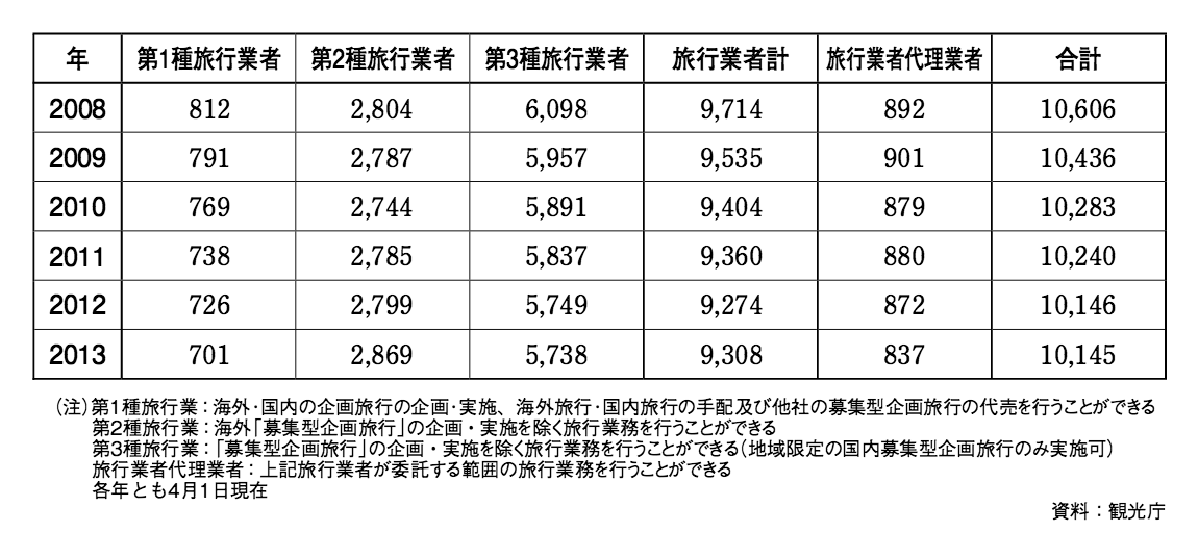
\includegraphics[scale=0.67]{tripgyosya.eps}
\end{center}
\caption{旅行業者数の推移}
\label{gyosya}
\end{figure}


旅行業者の取り扱い額も減少傾向にあり,国内旅行者は旅行業者を通じて旅行するのではなく,各々プランを立てて旅行する傾向になりつつあると考えられる.


\section{問題点} % sectionのタイトル
% 以下に背景,関連する環境,状況,技術に関する概要を記述.

個人旅行者が観光スケジュールを作成することは難しい.その理由として移動手段・時間を把握しにくいということ,様々な場所から探した情報をまとめる必要があること,視覚的にわかりやすく作成しにくいということが挙げられる.そのような問題を解決する手段の1つとして旅のしおり作成ツールが存在する.\\



\section{旅のしおり}
まず「しおり」とは「簡単な手引書や案内書」のことを指す.本研究では旅のしおりを「旅行の計画などを記録するツール」と定義する.\\
 単に観光スケジュールを作成するのではなく旅のしおりを作成することのメリットは,旅行前に旅行の計画を楽しみながら考えることができること,旅行後の振り返りとして他人と旅行の思い出の共有に使用できることが挙げられる.\\
 しかし既存の旅のしおりを作成するツールは観光スポットや移動手段・時間を手動で入力するものや,移動手段・時間を考慮せずに目的地をリスト的に表示するものが多い.そこで本研究では既存のツールを組み合わせ,移動手段・時間を考慮した旅のしおりによる観光スケジュール支援を行う.


\section{研究目的・目標}

本研究の目的は観光スケジュール作成を支援することである.この支援には二種類あり効率的に作成すること,楽しみながら作成することである.これらは必ずしも同時に満たす必要はなく,それぞれを独立に考える.その理由としては例を挙げると非効率的に時間をかけて旅行の計画を作成することに楽しさを覚える人もいるためである.よって楽しさと効率性の両面での支援を実現する必要がある.\\
 本研究の目標は「目的地と移動手段・時間が表示される旅のしおり作成ツールを開発する」である.


%--------------------------------------------------------------------
\chapter{関連研究}% 2章のタイトル

\section{CT-Planner}

本研究の関連研究としてWebサービスによる対話型の旅行計画支援ツール「CT-Planner」\cite{CTPlanner}がある(図2.1).

\begin{figure}[htpb]
\begin{center}
\includegraphics[scale=0.34]{ctplannner.eps}
\end{center}
\caption{CT-Planner}
\end{figure}

このツールは不慣れな土地での旅行計画作成に不安を抱く個人旅行者を対象としたものであり,函館や横浜などの都市を選択し「のんびり歩こう」「文化を知りたい」等の旅行スタイルの中から自分の嗜好に合ったものを選択すると,選択した旅行スタイルに応じた観光スポットを巡る旅行プランが自動的に作成される.旅行プラン作成後もユーザは行きたい観光スポットを適宜変更でき「穴場好き」か「有名所好き」等の特性を選ぶことでユーザの嗜好に合った旅行プランに変更できる.

%\subsubsection{必要があれば} % subsubsectionのタイトル
% ※ subsubsectionはあまり使わないほうがよい

\section{既存の旅のしおり作成ツール}

\subsection{電子的な旅のしおり作成ツールの例}
電子的な旅のしおり作成ツールには様々なものがあるが,代表して「ポケたび」\cite{poketrip}というツールについて記述する.ポケたびとはJTBが提供している旅のしおり作成ツールである.日本全国の観光スポットを検索することができ,そこから旅行プランを作成できる.またマルチデバイスに対応しておりPCの他にスマートフォンのアプリも存在する.

\subsection{紙媒体の旅のしおり作成ツールの例}
紙媒体の旅のしおり作成ツールには様々なものがあるが,代表して「TRAVELER'S notebook」\cite{traver}というツールについて記述する.このツールはTRAVELER'S COMPANYが販売する旅行の予定を記入できる手帳である.シンプルなデザインで旅行の予定や旅行中のことを自由に書き込むことができるスタイルとなっている.

\section{既存の乗り換え案内ツール}
既存の乗り換え案内ツールには様々なものがあるが,代表して「Yahoo!路線情報: 乗り換え案内」\cite{yahoo}というツールについて記述する.このツールはYahooが提供している,電車等の乗り換え案内を表示するツールである.このツールは,出発駅と到着駅を入力すると該当する路線や時刻や乗り換え案内情報を自動で表示する(図\ref{Lyahoo}).日時または曜日と時刻を指定することでより詳細に乗り換え案内が表示される.列車の乗り換え案内以外にも飛行機のや列車の運航状況や時刻表,路線図なども調べることが可能である.

\begin{figure}[htpb]
\begin{center}
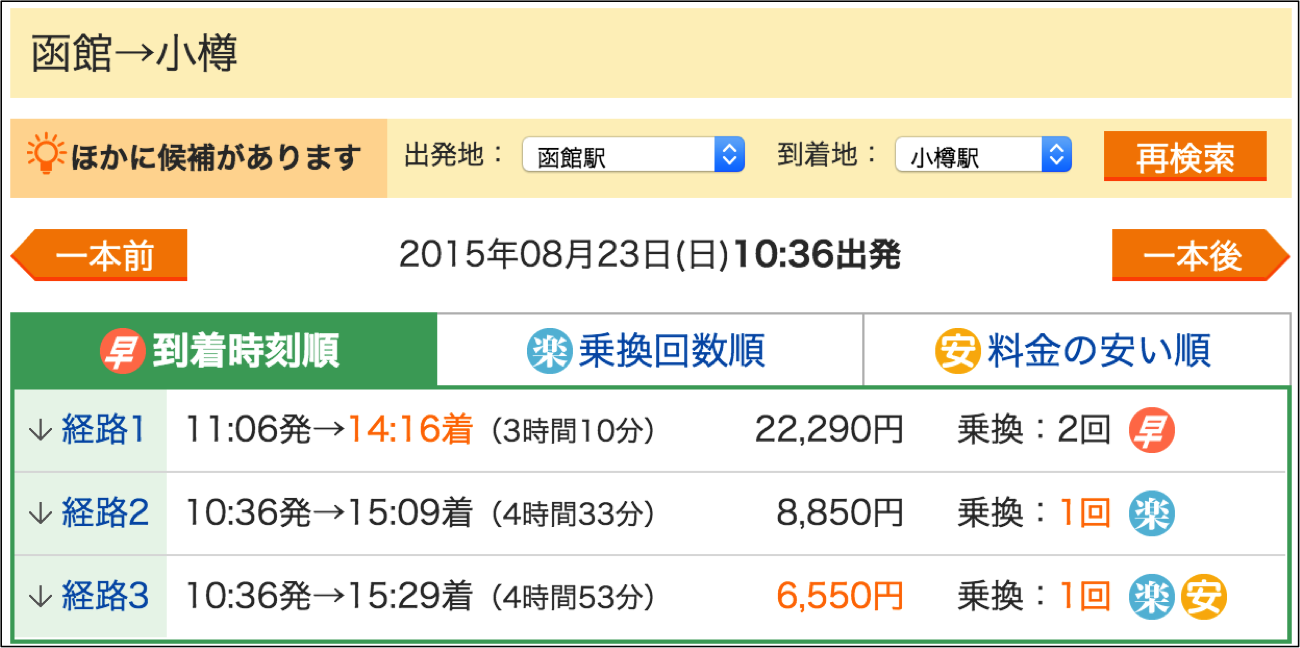
\includegraphics[scale=0.65]{yahoo.eps}
\end{center}
\caption{Yahoo!路線情報: 乗り換え案内}
\label{Lyahoo}
\end{figure}



%--------------------------------------------------------------------
\chapter{研究のアプローチ}% 3章のタイトル

本研究では始めに既存の旅のしおりの利点,問題点の調査を行った.次に旅行計画の作成についての考え方を知るために旅行計画作成に関するアンケートを行った.また,ツールを作成するうえで必要になる機能を調査するために予備実験を行った.その後,作成するツールの設計・実装を行う.

%\section{提案する言語FUNの特徴}

%この言語の特徴は,..であり,...という従来にない長所をもつ.

%\section{言語仕様}

%言語仕様は以下の通り.

%\section{実装方法}

%この言語は,C言語を用いて記述されている.ソースコードは20に分かれ,コードの大きさは約3000行となった.

%\subsection{開発環境}

%この言語は,C言語を用いて記述されている.ソースコードは20に分かれ,コードの大きさは約3000行となった.

%\subsection{OSに対する依存性}

%この言語は,C言語を用いて記述されている.ソースコードは20に分かれ,コードの大きさは約3000行となった.


%--------------------------------------------------------------------
\chapter{調査}% 4章のタイトル

既存でどのようなツールが存在するかを知るために既存の旅のしおり作成ツールの調査を行った.また旅行計画に対する考え方を知るためにアンケート調査を行った.


\section{既存の旅のしおり作成ツールの調査}

既存の旅のしおりは大きく分けて「観光スケジュールを作ることに重点を置いたツール」と「旅のしおりを作ることに重点を置いたツール」が存在する.\\
 1つ目の「観光スケジュールを作ることに重点を置いたツール」とは観光スポットや飲食店等をツールの内で検索し,自分の行きたい観光スポット等をスケジュールに組み込んで作っていくというものである.この例として「ポケたび」という旅行の計画を「旅のしおり」として作成・保存することができるツールがある.このツールでは旅行したい場所をエリアから選ぶまたは検索することで指定し,移動時間や滞在ホテルを指定することができる.また,このツールでは移動手段・時間は手動で入力する.\\
 2つ目の「旅のしおりを作ることに重点を置いたツール」とは印刷すると修学旅行等で作るような冊子のしおりになるものである.こちらはしおりの外面のデザインや写真といったことも決められるツールが多い.この例として「旅のしおり工房」\cite{tripkobo}という旅計画をたて「自分だけのガイドブック」をしおりにして持っていくことができるツールがある.このツールは始めに表紙の画像やデザインを決め,次に旅のテーマ,日程表などを作成していくことで冊子のしおりのように作ることができる.また,このツールでは旅行予定の場所や移動手段・時間は手動で入力する.\\
 上記の2つのツールは「観光スケジュールが作成できるか」「観光スポットが検索できるか」「移動手段・時間が表示されるか」「しおりのデザインが決定できるか」「マルチデバイスに対応しているか」の5つの観点で比較できると考えた.実際に比較を行った結果は表4.1のようになる.旅のしおり工房のマルチデバイス対応が△になっている理由は,携帯端末でも旅のしおり工房のWebページを開きしおりを作成することは可能であるが,PCと携帯端末でしおりの共有ができないためである.

\begin{table}[htb]
\begin{center}
\caption{既存の旅のしおり作成ツールの比較}
  \begin{tabular}{|c|p{2.0cm}|p{2.0cm}|p{2.0cm}|p{2.0cm}|p{2.0cm}|} \hline
     & 観光スケジュールの作成 & 観光スポットの検索 & 移動手段・時間の自動表示 & しおりのデザインの決定 & マルチデバイス対応 \\ \hline 
    ポケたび & ○ & ○ & × & × & ○ \\ \hline
    旅のしおり工房 & ○ & × & × & ○ & △\\ \hline
  \end{tabular}
  \end{center}
\end{table}


この調査から既存の旅のしおり作成ツールでは移動手段・時間を手動で入力しなければならないということがわかった.また既存の旅のしおりには表4.1にある5つの項目が搭載されており,作成するツールにもそれらが必要になるということもわかった.\\



\section{旅行計画作成に関するアンケート}
次に本学の学生,教員,事務員に対して旅行計画作成に関するアンケートを行った.52人にアンケートの回答を依頼したところ19人から回答があった.\\

\subsection{回答者の属性}
回答者の年代の割合は20代が58\%,30代が16\%,40代が21\%,50代が5\%となった(図\ref{Lnendai}).

\begin{figure}[htpb]
\begin{center}
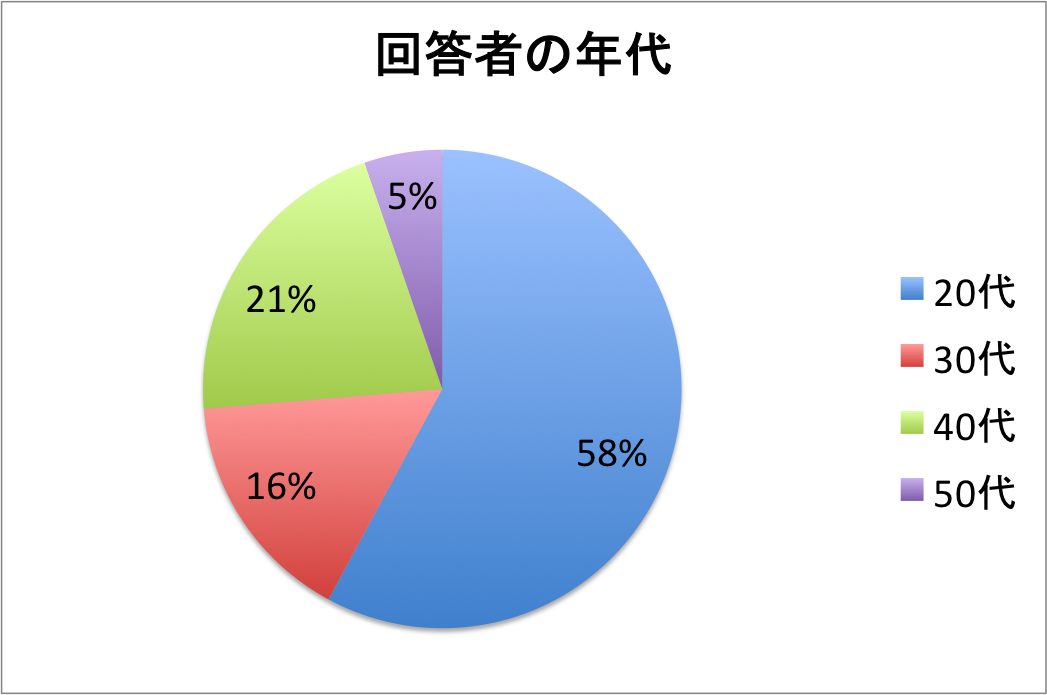
\includegraphics[scale=0.65]{nendai.eps}
\end{center}
\caption{回答者の年代の割合}
\label{Lnendai}
\end{figure}

\clearpage

次に回答者における男性の割合は68\%,女性の割合は32\%となった(図\ref{Lgender}).

\begin{figure}[htpb]
\begin{center}
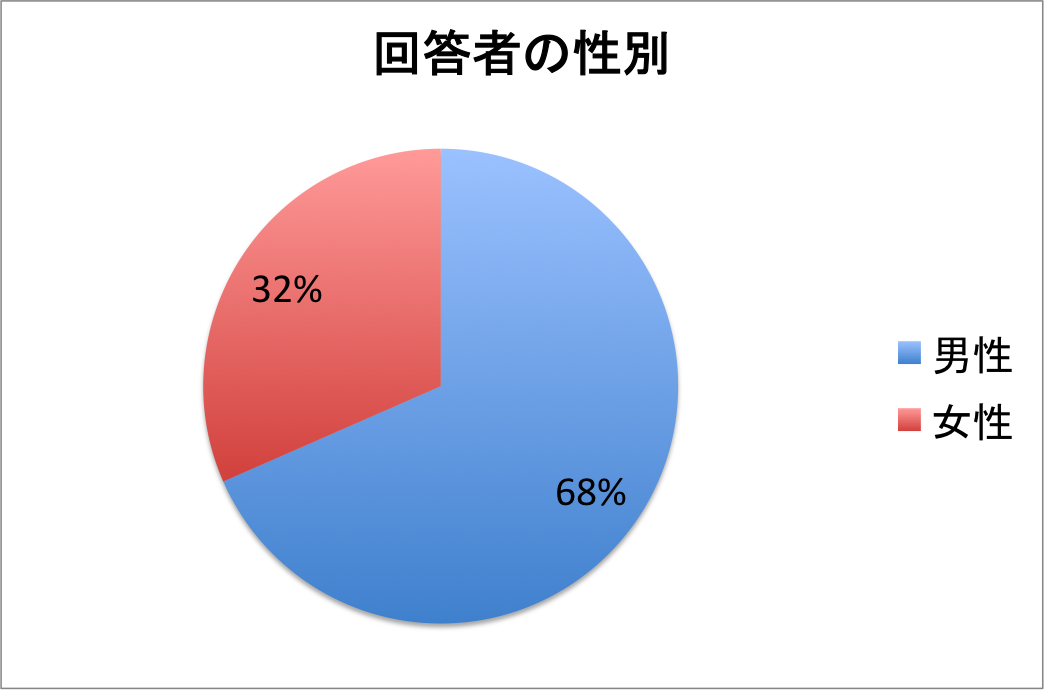
\includegraphics[scale=0.65]{gender.eps}
\end{center}
\caption{回答者の性別の割合}
\label{Lgender}
\end{figure}

\clearpage

最後に回答者における職業の割合は学生が63\%,教員が26\%,事務員が11\%となった(図\ref{Ljob}).

\begin{figure}[htpb]
\begin{center}
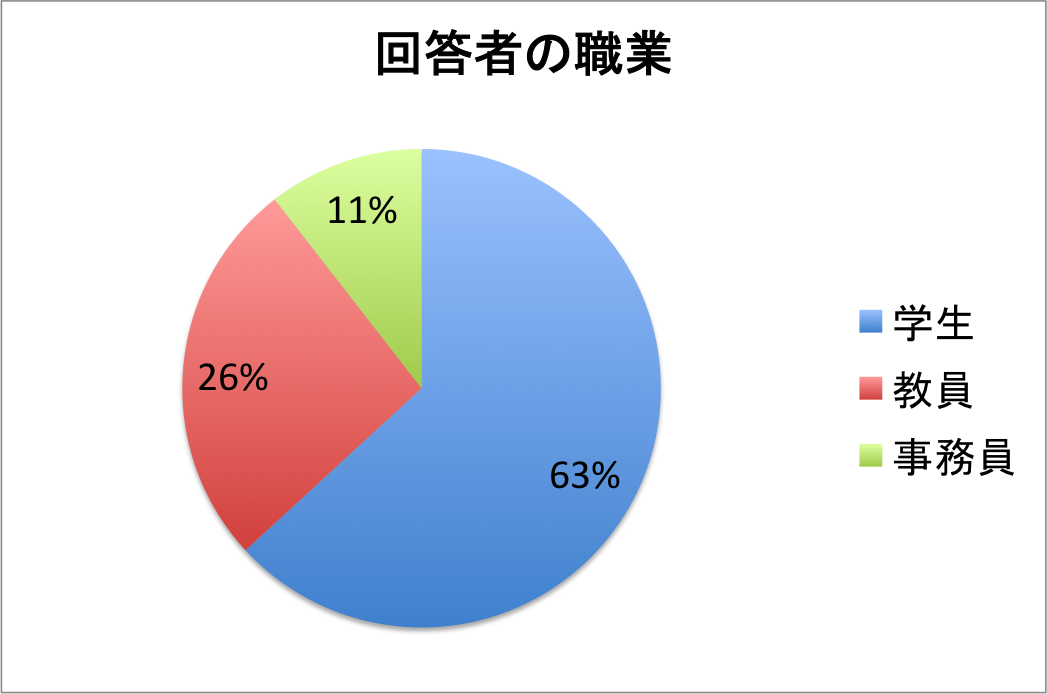
\includegraphics[scale=0.65]{job.eps}
\end{center}
\caption{回答者の職業の割合}
\label{Ljob}
\end{figure}

\clearpage

\subsection{旅行の頻度と計画作成方法}

「1年間に出張(公務旅行を含む)は何回ほど行きますか」という質問に対して「4回以下」という回答が68\%を占めた(図\ref{Lsyutyo}).

\begin{figure}[htpb]
\begin{center}
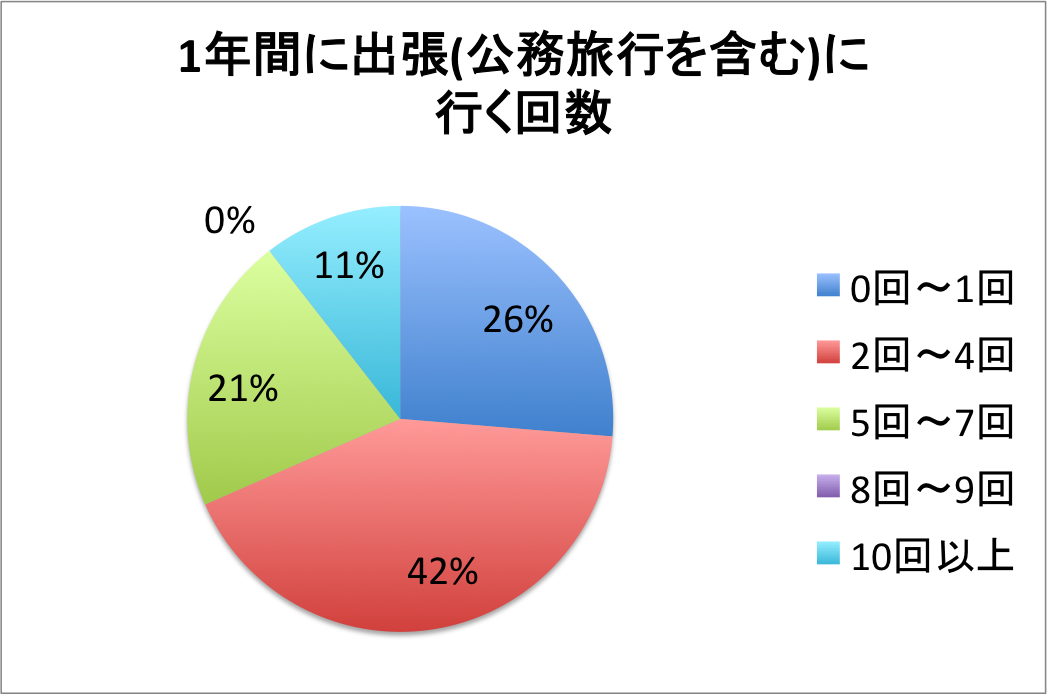
\includegraphics[scale=0.65]{syutyo.eps}
\end{center}
\caption{1年間に出張(公務旅行を含む)に行く回数}
\label{Lsyutyo}
\end{figure}

\clearpage

「仕事以外の旅行は1年間に何回ほど行きますか」という質問に対して「4回以下」という回答が84\%を占めた(図\ref{Lcryoko}).

\begin{figure}[htpb]
\begin{center}
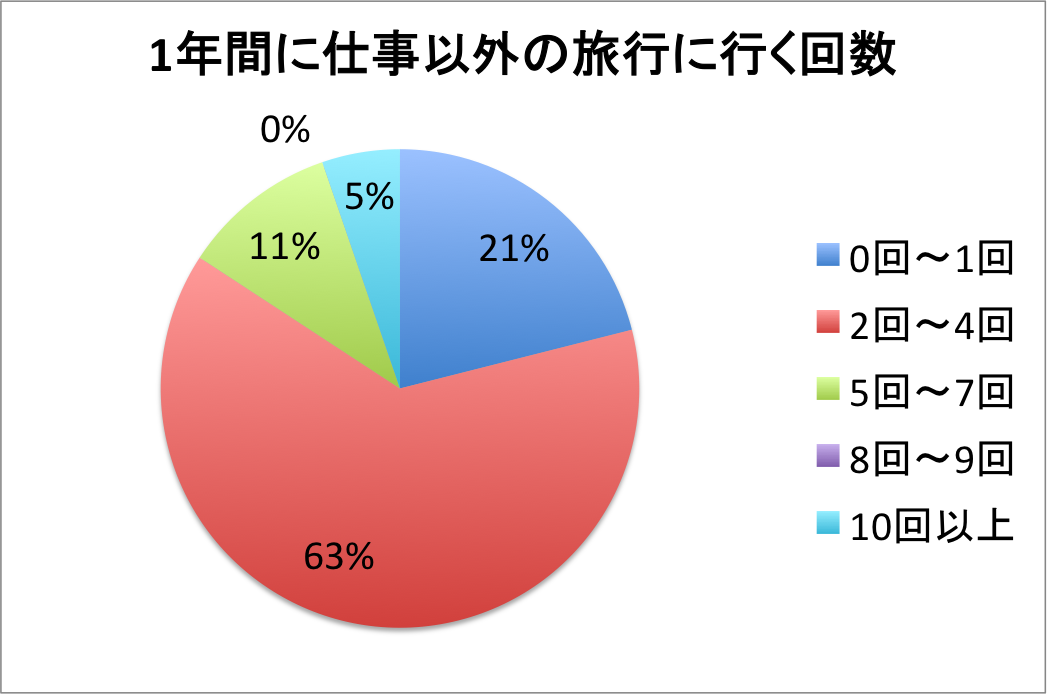
\includegraphics[scale=0.65]{cryoko.eps}
\end{center}
\caption{1年間に仕事以外に旅行に行く回数}
\label{Lcryoko}
\end{figure}

\clearpage

「出張の旅行の際,空き時間等に観光することはありますか」という質問に対して「よくある」と「少しはある」という回答が82\%を占めた(図\ref{Lakitime}).

\begin{figure}[htpb]
\begin{center}
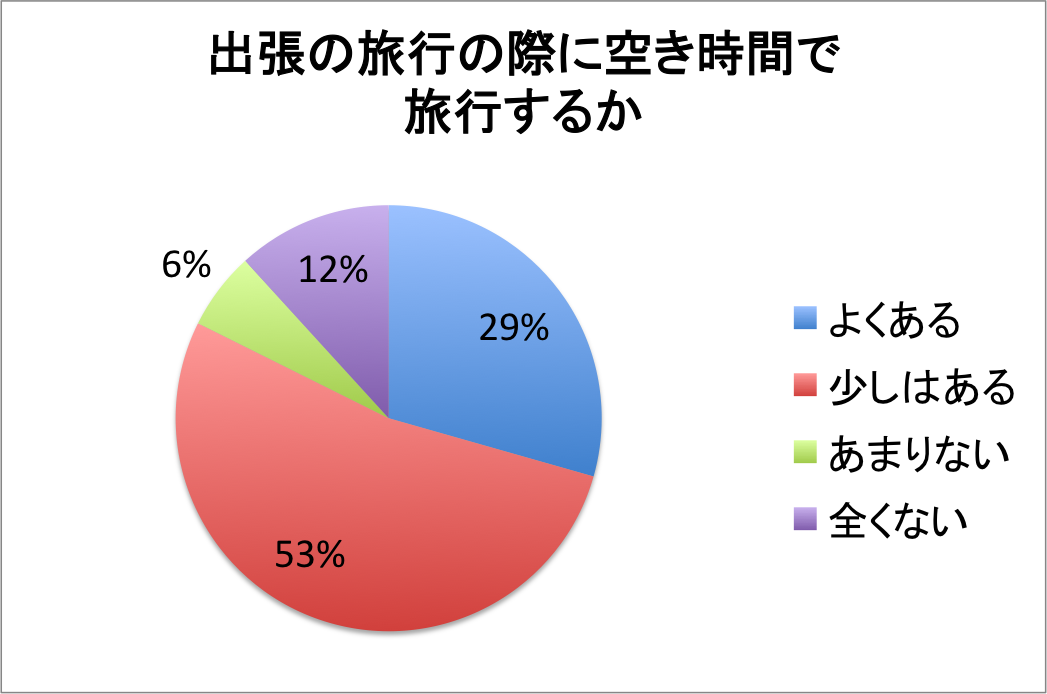
\includegraphics[scale=0.65]{akitime.eps}
\end{center}
\caption{空き時間に観光することがあるか}
\label{Lakitime}
\end{figure}

\clearpage

「出張の旅行の際によく使用するWebサイトを選択してください(複数回答可)」という質問に対して「航空会社のWebサイト(もしくはアプリ)」が最も多く13票,次点で「乗換案内サイト(ジョルダン,駅すぱあと,駅探等)」と「ルート検索サイト(Google Maps等)」が12票であった(図\ref{Lwebsyutyo}).

\begin{figure}[htpb]
\begin{center}
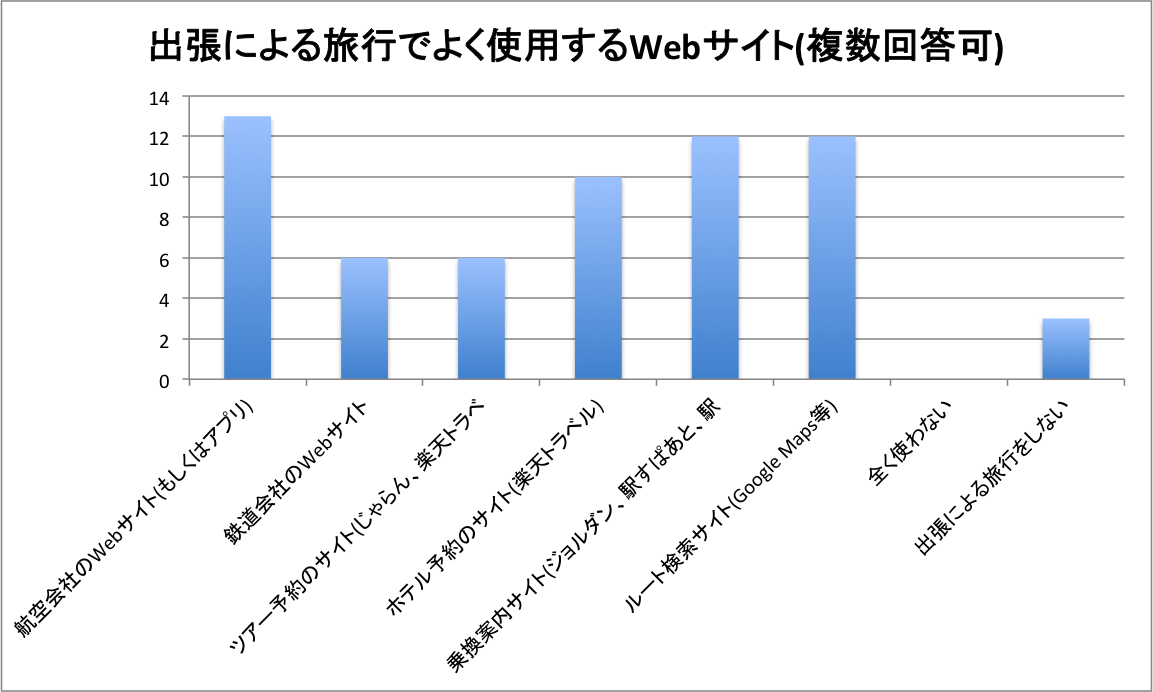
\includegraphics[scale=0.7]{websyutyo.eps}
\end{center}
\caption{出張による旅行でよく使用するWebサイト(複数回答可)}
\label{Lwebsyutyo}
\end{figure}

またその他に使用するサイトとして
\begin{itemize}
 \item デパートの旅行代理店
 \item 食べログ
 \item バス停検索サイト
 \item 出張先でググる
\end{itemize}
という回答があった.

\clearpage

「観光のみの旅行の際によく使用するWebサイトを選択してください(複数回答可)」という質問に対して「ホテル予約のサイト(楽天トラベル)」と「ルート検索サイト(Google Maps等)」が最も多く9票であった(図\ref{Lwebtrip}).

\begin{figure}[htpb]
\begin{center}
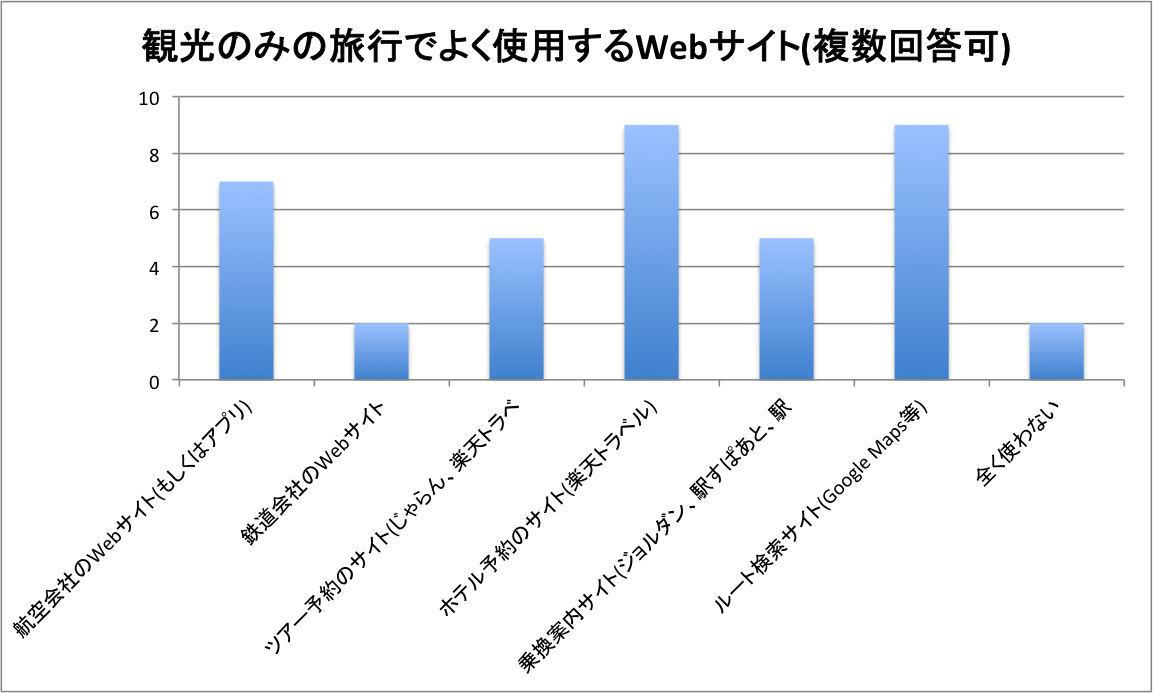
\includegraphics[scale=0.7]{webtrip.eps}
\end{center}
\caption{観光のみの旅行でよく使用するWebサイト(複数回答可)}
\label{Lwebtrip}
\end{figure}


またその他に使用するWebサイトとして
\begin{itemize}
 \item レンタカーのサイト
 \item 公式観光情報サイト
 \item 出張先でググる
 \item 旅先の気候や気温がわかるサイト
 \item 地域の観光ページ
 \item 特産品のページ
 \item Facebookの口コミ
 \item (Webサイトではないが)ガイドブック
\end{itemize}
という回答があった.

\clearpage

「旅行計画を作成する際にオススメのWebサイトを教えてください」という質問に対しては
\begin{itemize}
 \item 特定のサイトではないが,乗換案内サイトなどはサイトによって対応している交通機関が多少異なったりするので,行き先や状況に応じて同じ種類の異なるサイトを使い分けたり,並行して使ったりする
 \item 観光客向けのおすすめコースやスポット(Webサイトや紙媒体のマップ)
 \item NAVERまとめ物語のように記事が書かれている場合もあるので,そうゆう場合読みやすい
 \item 各地域のデパートの地下に地域特産品が売っていることが多いので,まず地図を検索して宿泊先を決める,確認する.そしてその近くにあるデパートを探す→定休日でないか調べる→お店を確認する,食べログなどでレビューを見る・・・
 \item 美術館や博物館が好きなので,旅行期間で開催されている展覧会の情報をネットを巡って調べる→場所・交通手段を確認する,定休日でないか調べる
 \item バス停検索
 \item トレッキングのサイト
\end{itemize}
という回答があった.

\clearpage

\subsection{旅行の記録方法}

 「旅行前に旅行の計画を紙やファイルなどをどこかに記録するか」という質問に対して「計画を立てて記録する」が56\%,「計画を立てるが記録しない」が33\%,計画を立てないが11\%であった(図\ref{Lfilerecord}).

\begin{figure}[htpb]
\begin{center}
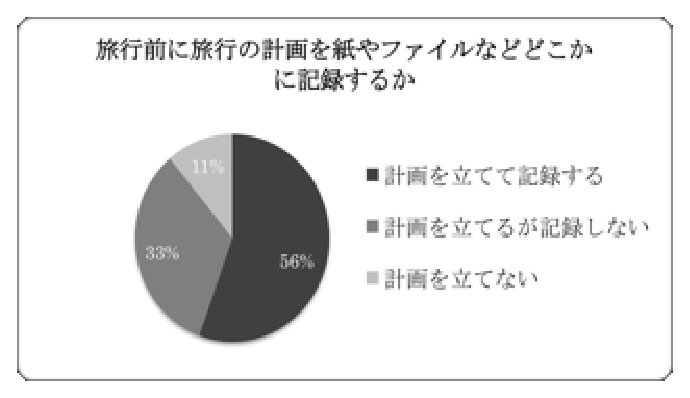
\includegraphics[scale=0.65]{filerecord.eps}
\end{center}
\caption{旅行前に計画を記録するか}
\label{Lfilerecord}
\end{figure}

「計画を立てて記録する」と回答した方に記録する方法を記入してもらったところ,以下のような回答を得た.
\begin{itemize}
 \item 紙
 \item Word
 \item googleドライブ
 \item evernote
 \item 手帳
\end{itemize}


「計画を立てるが記録しない」と回答した方にその理由を記入してもらったところ,以下のような回答を得た.
\begin{itemize}
 \item めんどくさい
 \item 計画通りに進まないことがあるから.おおまかな計画はたてるが,その場でスマートフォン等で検索する
 \item 計画は立てた方がいいが,記録が面倒だから
 \item 記録する必要がないため
 \item Webページを利用して予約等行うとそこに記録が残るから
 \item 記録するほど綿密に計画を立てない
\end{itemize}


\subsection{他人との共有方法}

「旅行前に旅行の計画を誰かに話すか」という質問に対して「はい」は84\%「いいえ」は11\%「旅行の計画を立てない」が5\%であった(図\ref{Lbeforetalktrip}).\\
\begin{figure}[htpb]
\begin{center}
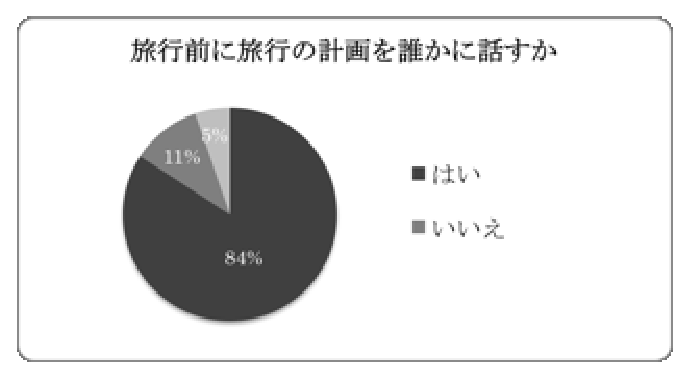
\includegraphics[scale=0.65]{beforetalktrip.eps}
\end{center}
\caption{旅行前に計画を話すか}
\label{Lbeforetalktrip}
\end{figure}


「旅行前に計画を誰かに話す」と回答した方に,どんな立場の相手にどのような手段で伝えるか記述してもらったところ,以下のような回答を得た.
\begin{itemize}
 \item 友人にLineかtwitterで伝える
 \item 旅行の同行者にメールで連絡
 \item 口頭で大まかなスケジュールを伝える
 \item 旅行の同伴者にはメールなどで伝える
 \item 基本的に旅行の同行者にメールやGoogleドライブ上のファイルで共有
 \item 出張時の旅程もGoogleドライブ上の共有ファイルで大まかに家族と共有
 \item 友人に口頭で
 \item 家族に電話やメールで連絡
 \item 業務の旅行だったら事務局へ旅行伺書を提出する.個人の旅行だったら誰にも伝えない
 \item 同行者と調べた情報を共有.家族に目的地(用務先),ホテル,飛行機や鉄道の便を通知
 \item 旅行の同行者にGoogleカレンダーやメールで共有
 \item 複数人の旅行で,自分がホテルの予約を行った場合は,LINEで伝える
 \item 家族もしくは親族にメールもしくは紙で連絡
 \item 家族に電話で連絡
 \item 家族にテキストチャット(iMessage)で連絡
\end{itemize}

\clearpage

「旅行後に旅行の計画を誰かに話すか」という質問に対して「はい」は32\%「いいえ」は63\%「旅行の計画を立てない」が5\%であった(図\ref{Laftertalktrip}).

\begin{figure}[htpb]
\begin{center}
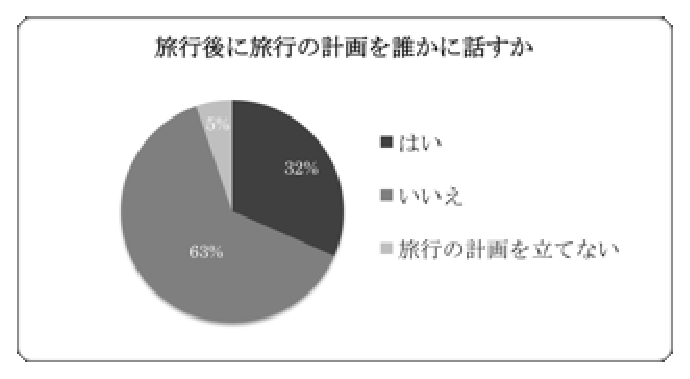
\includegraphics[scale=0.65]{aftertalktrip.eps}
\end{center}
\caption{旅行後に計画を話すか}
\label{Laftertalktrip}
\end{figure}


「旅行後に計画を誰かに話す」と回答した方に,どんな立場の相手にどのような手段で伝えるか記述してもらったところ,以下のような回答を得た.
\begin{itemize}
 \item 友人にお土産ついでに伝える
 \item 詳しい計画を伝えることはないですが,どこに行ったかなんとなく分かる程度にFacebookにアップしたりすることはある
 \item 友人に口頭で
 \item 家族に無事帰宅した旨を電話やメールで連絡
 \item 同行者に無事帰宅した旨を電話やメールで連絡
 \item 喋っていい内容であればFacebookに旅行で撮った写真をアップする.詳細なスケジュールは載せない
 \item 伝えるというよりは,twitterなどのSNSに上げることが多い
\end{itemize}



\subsection{旅行計画作成の印象}

「旅行の計画を立てることをどう思うか(複数回答可)」という質問に対して,「楽しい」という回答が最も多く次点で「面倒」「わくわくする」「自分で立てたい」が続いた(図\ref{Lhowthinktrip}).

\clearpage

\begin{figure}[htpb]
\begin{center}
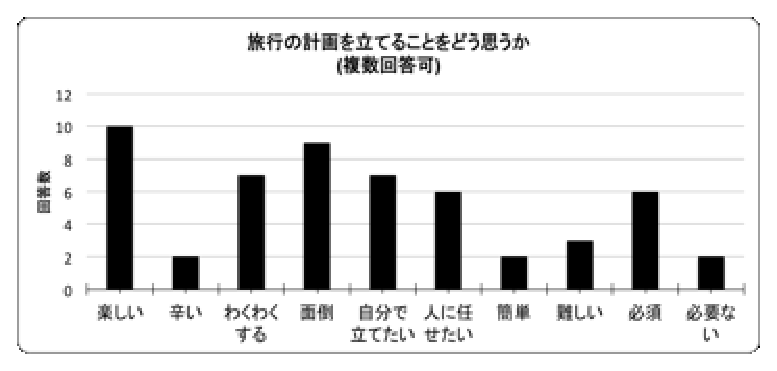
\includegraphics[scale=0.7]{howthinktrip.eps}
\end{center}
\caption{旅行計画を立てることをどう思うか}
\label{Lhowthinktrip}
\end{figure}

これらの結果から,旅行の計画を立てる人は多く,旅行前に計画を話すということも行われることが多いとわかった.また,旅行計画を立てることに楽しさを感じる人が多いが,面倒だと感じる人も多い.そのためツールで楽しさを感じてもらいつつ,面倒さを解消することが必要になる.\\



\section{考察}
調査によって既存の旅のしおりには観光スポットまたは移動時間を手動で入力するものや移動手段を考慮せずに目的地をリスト的に表示するものが多いという問題点があることがわかった.そのため移動手段・時間を自動的に表示することでより作成するツールの利便性が高まると考えられる.
また,今回比較に使用した「観光スケジュールの作成」「観光スポットの検索」「移動手段・時間の自動表示」「しおりのデザインの決定」「マルチデバイス対応」の5つの観点のうち,全てではなくてもいくつか満たされていることで「旅のしおり」になるということが考えられる.そのため,開発するツールでは可能な限りこれら5つの観点は盛り込まれているべきであると考える.\\
 次にアンケート結果によって出張等の空き時間に観光する人が多いとわかった.これよりそれほど多くない空いた時間に素早く計画を立てることができる工夫があると,より利便性が高まると考えられる.出張の旅行と観光の旅行では使用するWebサイトに若干の違いが見られた.出張において航空会社のWebサイトが多く使用されているのは回答者が函館という地方都市に在住していることも影響していると考えられる.ルート検索サイトはどちらの場合でも使用している人が多いとわかった.これは馴染みの薄い土地に行く際には多くの人がルート案内サイトを使って経路を調べているからであると考えられる.観光による旅行では公式の観光情報サイトや特産品のサイトでより詳しい情報を得ようとしたり,レンタカーのサイトで移動手段を確保する人もいるとわかった.行きたい土地の観光スポットがまとまっているサイトを利用しているという回答もあった.これは多くの選択肢の中から自分の行きたい場所を選ぶことができるため,様々なサイトを移動する必要がないと考えられる.こういった選択の幅を広げる工夫は開発するツールでも取り入れるべきである.旅行計画の記録に関しては計画自体を立てる人は約9割であったが,記録までする人は約5割であった.記録しない人の考えとして,面倒ということやその場で考えるという回答があった.面倒という感情については後ほど詳しく考察する.
複数人で行く場合は同伴者に事前に話す人が84\%であった.伝える方法としては口頭やメールなどが多いため,旅のしおり作成ツールによって他人とも共有できることで,利便性が高まると考えられる.旅行後はスケジュールを話すのではなく,旅行の経験や体験をお土産話として友人などに伝えるという回答があった.そのため,開発するツールではスケジュールを立てることだけを支援するのではなく,旅行の想い出を残す機能も必要であると考えられる.最後に旅行計画を立てることに関しては「楽しい」という回答と「面倒」という回答が多かった.「楽しい」という感情に寒鴉してはこれから行く旅行のことをあれこれ考えながら計画を立てることを楽しんでいると考えられる.逆に面倒と感じる要因としては自分の必要としている情報がなかなか手に入らないことや,細かく記録を残すことを億劫に思う感情があると考えられる.よって開発するツールには面倒さを解消することと,楽しさを感じることができる要素が必要である.どのような場面で楽しさを感じているかということはこのアンケート結果だけでは不確かであったため,更に詳しく調べる必要があると考えられる.


%--------------------------------------------------------------------
\chapter{予備実験}% 5章のタイトル
ツールを作成するうえで必要になる機能,特に「楽しさ」という観点で見た場合にどのような要素が必要になるかということや,どのような場面でユーザは「楽しさ」を感じているかということを調べるために予備実験を行った.

\section{実験計画}
この予備実験を計画する際に本学の認知科学に詳しい教員にアドバイスをいただいた.その内容は「被験者は1名ではなく2名で行ってもらい,その2名も可能であれば実際に旅行に行くような間柄の関係の人にすべき」,「複数の案から選択できるような形式にする」,「被験者の発言内容,表情,口調などから読み取れることがある」というものであった.そこで予備実験の方法として,被験者2名ずつペアになってもらい,こちらが数パターン用意した旅行計画の概要の中から行きたいというものを選んでもらう.また既存のツールを用いて実際に旅行計画を立ててもらうものである(図5.1).
\begin{figure}[htpb]
\begin{center}
%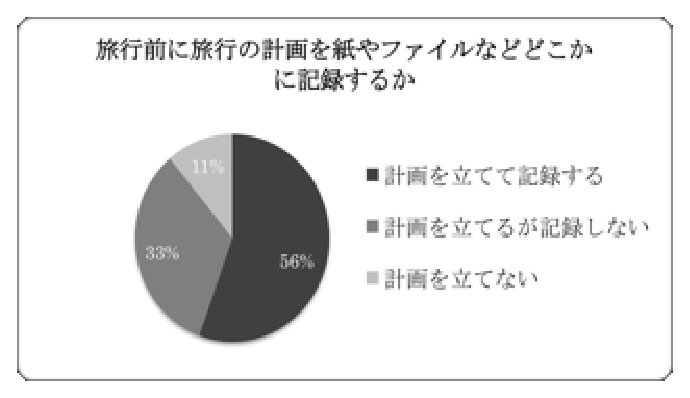
\includegraphics[width=4cm, height=2cm]{filerecord.eps}
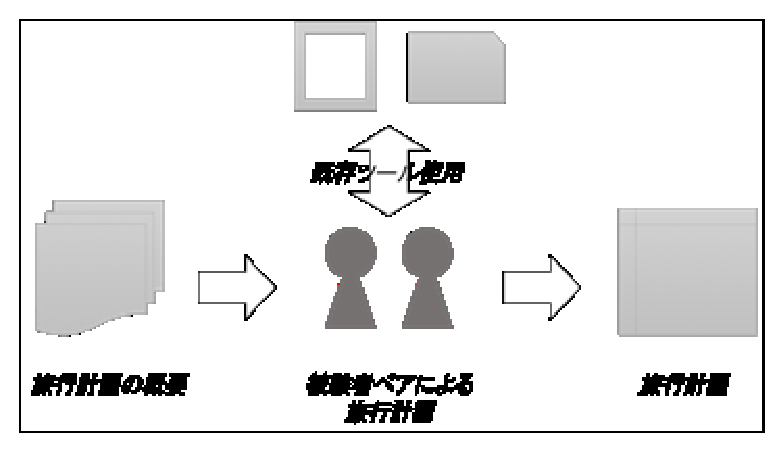
\includegraphics[scale=0.4]{semiexp.eps}
\end{center}
\caption{予備実験イメージ}
\end{figure}


\section{実験概要}
本学の学部4年2名を被験者として実験を行った.こちらからは「卒業旅行を想定すること」「旅行の期間は2泊3日とすること」の2点を指定した.
被験者はPCを使って旅のしおりを作成することとし,ツールは「ポケたび」を使用することとした.また旅のしおりを作成する際にはポケ旅以外のWebのサイトは自由に使用して構わないとした.
実験中は画面をと音声を収録した.また終了後にインタビューを実施した.

\section{実験結果}
まず被験者はどこに行くかを決めるための話し合いを始めた.実験の様子は図5.2の通りである.

\begin{figure}[htpb]
\begin{center}
%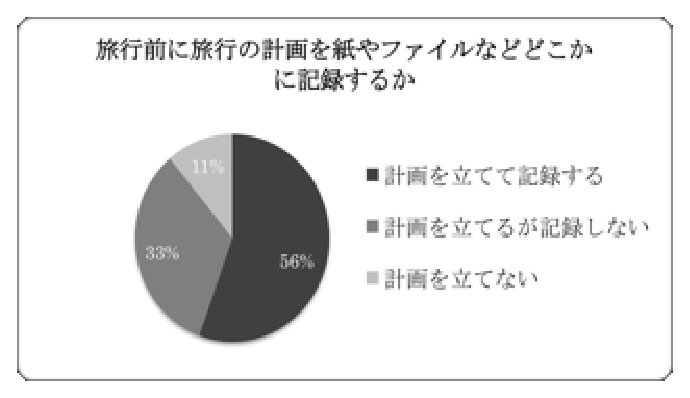
\includegraphics[width=4cm, height=2cm]{filerecord.eps}
\includegraphics[scale=0.09]{expfoto.eps}
\caption{予備実験の様子}
\end{center}
\end{figure}


最初にユニバーサル・スタジオ・ジャパン(以下USJ)に行きたいと話し合い,USJの場所を調べ始めた.その際USJの公式Webサイトを使用していた.しかし,最初から候補を絞りすぎるのはよくないと考え箱根や沖縄といった地名をあげていった.少しの話し合いの後にとりあえず,ポケたびのお気に入り機能を使って気になる観光スポットを登録する作業を始めた.まずは大阪のおすすめ観光スポットを紹介しているWebサイトを調べた.そこで,USJ,海遊館,天保アニパ,天王寺動物園という観光スポットの候補を発見した.被験者にとってUSJと海遊館は馴染みのある場所であったが,天保アニパと天王寺動物園については詳しく知らなかったため,その2つの観光スポットについてWebサイトで詳しく調べ始めた.またその際に海遊館の詳しい場所も海遊館のWebサイトにて調べていた.海遊館などをお気に入りに指定する際にポケたびの検索機能を用いてスポットを探していた.
次に大阪のグルメについて,グルメ情報サイトで調べ始めた.その際,先ほどと同じようにポケたびのお気に入り機能を使用して行きたい思った候補地を記録していた.次におおよそ大阪近辺を観光することが決まったため,大阪府内での交通手段を調べ始めた,その際,乗り換え案内のサイトなどを利用して交通手段を調べていた.その後,滞在するホテルを宿泊料金を比較できるサイトにて調べていた.場所や料金の適するホテルを見つけ,そのホテルのサイトにて詳細を調べていた.飛行機の時間や料金などはこの段階で調査をしていた.その際,函館空港と伊丹空港のWebページを参照していた.また伊丹空港からの交通手段を乗り換え案内サイト等を使用して調べていた.
それが終わると旅のしおり作成を開始した.旅のしおりを作成する際にはそれまでにお気に入りに入れたスポットを参照しながら,しおりを丁寧に作成し始めた.作成開始当初は場所の指定や手動で場所を入力する方法に戸惑っている様子が見られた.飛行機や列車の時間を記入する際は調べる段階で開いておいたWebサイトを見返したり,必要に応じて新しく調べたりしていた.また,ホテルの場所や食事の場所も先ほど調べた情報を参照したり,新しく調べたりして記入していた.実験中に



最後にインタビューを実施し,今回の実験の感想などを聞いた.実際に被験者が作成した旅のしおりを以下に示す.(図5.2),(図5.3),(図5.4)\\

\begin{figure}[htpb]
\begin{center}
%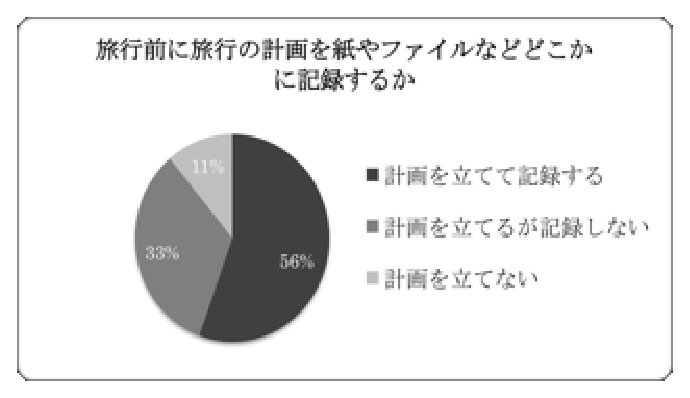
\includegraphics[width=4cm, height=2cm]{filerecord.eps}
\includegraphics[scale=0.7]{shiori1.eps}
\caption{実験で被験者が作成したしおり(1/3)}
\end{center}
\end{figure}

\begin{figure}[htpb]
\begin{center}
%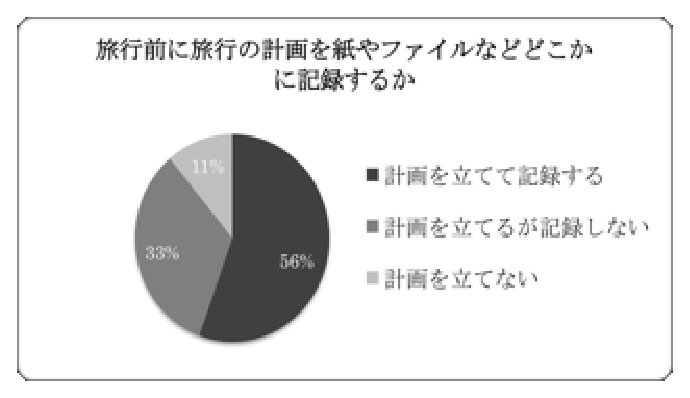
\includegraphics[width=4cm, height=2cm]{filerecord.eps}
\includegraphics[scale=0.7]{shiori2.eps}
\caption{実験で被験者が作成したしおり(2/3)}
\end{center}
\end{figure}

\begin{figure}[htpb]
\begin{center}
%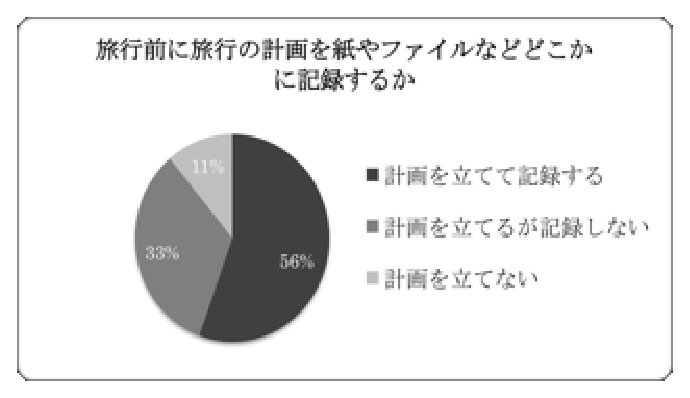
\includegraphics[width=4cm, height=2cm]{filerecord.eps}
\includegraphics[scale=0.7]{shiori3.eps}
\caption{実験で被験者が作成したしおり(3/3)}
\end{center}
\end{figure}


 被験者の表情の観察から,行き先を決めるために様々な場所を候補地として探している時間が楽しそうにしていた.実験後のインタビューでは旅行計画を作成することと使用したツールについて聞いた.被験者は1時間かけて旅のしおりを作成した.1時間の内訳は始めの30分を目的地を決める時間に使用し,残りの30分間を旅のしおりを作成する時間に使用していた.\\
 旅行計画を作成することでは「自分が行きたい場所のことを考えるのは楽しい」「実際に旅行する場面を思い描きながら作成できて良かった」などの意見があった.また「しおりという形に残るものがあると,より楽しさが深まりそう」という意見もあり,これは開発するツールに取り入れるべき意見であった.\\
 使用したツールに関してはポケたびを利用して気になった点を挙げてもらった.具体的には「ブラウザの戻るボタンを押すのではなく,ポケたび内の戻るボタンを押さなくてはならない」「アイコンではなく右のチェックマークをクリックする必要があるが,アイコンをクリックしてしまう.」などがあった.良かった点としては「観光スポットを検索できる」「お気に入り機能がある.」などがあった.またあったら良いと思う機能としては「移動時間や・手段を自動で表示する」「目的地の経路を表示する」ということがあった.

\section{考察}
本研究で開発するツールではこれらの要素が満たされることで,効率性や楽しさの面での支援が期待できることがわかった.被験者が最も楽しさを感じている場面は,実験中の様子から見て目的地を決めるために,
観光スポットを検索している時間であった.また実験の旅行計画を作成する段階の終盤では若干飽きや面倒さを感じていたように見えた.理由として始めは移動手段・時間等を細かく記入していたものの,最後の方では雑に記入している様子が見られた.開発するツールでは旅のしおりを作成する際の面倒さを減らす必要があると改めてわかった.「ポケたび」のUIの面で誤認識をしてしまう場面があったため,作成する



%--------------------------------------------------------------------
\chapter{作成するツール}% 6章のタイトル

現時点ではツールの構成イメージとしてAPI等を用いて地図や乗り換え案内,ルート検索などのツールと組み合わせ移動手段・時間を表示する(図6.1).
\begin{figure}[htpb]
\begin{center}
%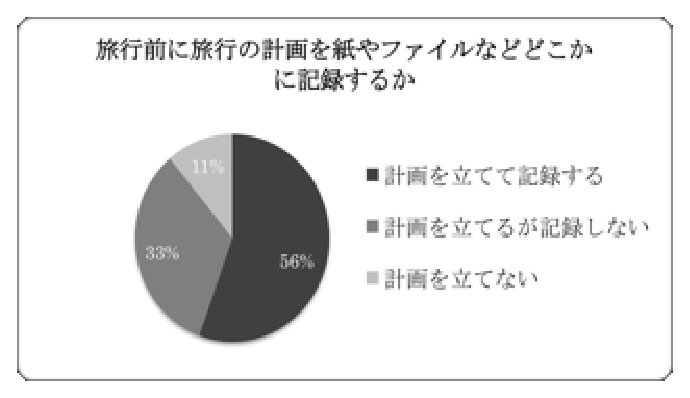
\includegraphics[width=4cm, height=2cm]{filerecord.eps}
\includegraphics[scale=0.4]{willmaketools2.eps}
\caption{作成ツールイメージ}
\end{center}
\end{figure}

最終版では加筆します.

%--------------------------------------------------------------------
\chapter{結論と今後の展開}% 7章のタイトル

\section{まとめ}

本研究ではツールを組み合わせ,移動手段・時間を考慮した旅のしおりによる観光スケジュール支援を行う.現段階では既存のツールと旅行計画作成の考え方の調査を行い,既存の旅のしおり作成ツールは移動手段・時間を考慮していないこと,旅行計画を立てる人の割合が多いこと,旅行計画作成について「楽しい」「面倒」と考える人が多いことがわかった.\\



\section{今後の展開}
今後加筆します.
 %今後はユーザが旅のしおりを作成するうえで「楽しさ」を感じてもらうためにはどのようなことが必要になるかということや,そのことを踏まえて必要機能の検討とツールの設計,実装を行う.



%--------------------------------------------------------------------
\chapter*{謝辞}
本研究に対して様々な指導や的確なアドバイスをしてくださった,伊藤恵先生に深くお礼を申し上げます.また,ゼミの中で様々な助言をしてくださった,研究室のメンバー,ご助言をいただいた南部先生,発表会の場でご質問ご指摘してくださった先生や学生の皆様に心から感謝致します.また,本研究にご指摘くださった観光情報学会並びにFOSE2105参加者の皆様にも深くお礼を申し上げます.



%--------------------------------------------------------------------
% 参考文献
\begin{thebibliography}{9}
\bibitem{kokunaitrip}日本交通公社,日本の国内旅行  {\url{https://www.jtb.or.jp/wp-content/uploads/2015/10/nenpo2015_1-2.pdf}}, 参照(2016-1-23)
\bibitem{ryokougyokai}日本旅行業協会,数字が語る旅行業2014  {\url{https://www.jata-net.or.jp/data/stats/2014/pdf/2014_sujryoko.pdf}}, 参照(2016-1-23)
 \bibitem{CTPlanner} 倉田陽平ら,旅行プラン作成ツールCT-Plannerのプラットフォーム化に向けて,観光情報学会第11回全国大会,pp.38-39,2014
\bibitem{poketrip}ポケたび,  {\url{https://poketabi.com/}}, 参照(2015-12-20)
\bibitem{traver}TRAVELER'S COMPANY -JAPAN-,  {\url{http://www.travelers-company.com/products/trnote/about}}, 参照(2016-1-13)
\bibitem{yahoo}Yahoo!路線情報: 乗り換え案内,  {\url{http://transit.loco.yahoo.co.jp/}}, 参照(2016-1-13)
\bibitem{tripkobo}旅のしおり工房,  {\url{https://www.mapfan.com/shiori/}}, 参照(2015-12-20)
\bibitem{tt} 辻浦崇大ら,移動手段・時間を考慮した旅のしおりによる観光スケジュール作成支援旅行プラン作成ツール,観光情報学会第11回研究発表会,2015

\end{thebibliography}


% 以降,付録(付属資料)であることを示す
\appendix

%--------------------------------------------------------------------
%\chapter*{付録その1} % \chapter{}を使うと「付録A ***」となる

%付録その1(プログラムのソースリストなど)を必要があれば載せる

%--------------------------------------------------------------------
\chapter*{付録その1}

\begin{figure}[htpb]
\begin{center}
%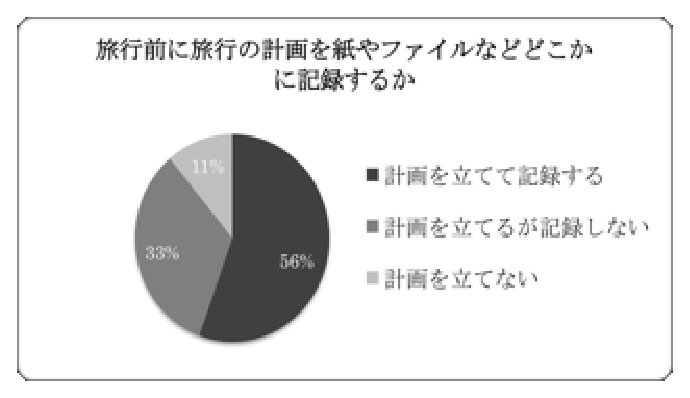
\includegraphics[width=4cm, height=2cm]{filerecord.eps}
\includegraphics[scale=0.7]{ank1.eps}
\caption{旅行計画に関するアンケート(1/6)}
\end{center}
\end{figure}

\begin{figure}[htpb]
\begin{center}
%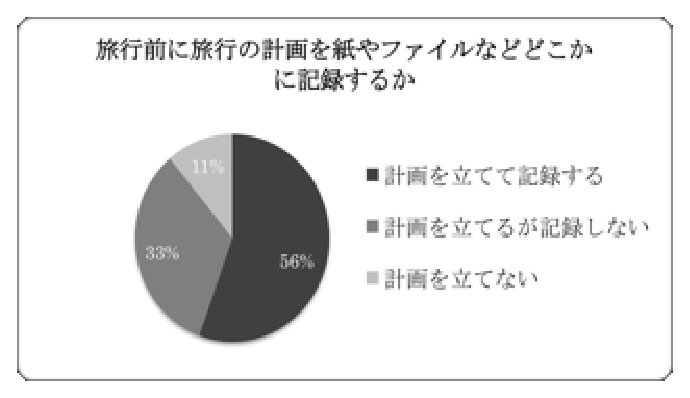
\includegraphics[width=4cm, height=2cm]{filerecord.eps}
\includegraphics[scale=0.7]{ank2.eps}
\caption{旅行計画に関するアンケート(2/6)}
\end{center}
\end{figure}

\begin{figure}[htpb]
\begin{center}
%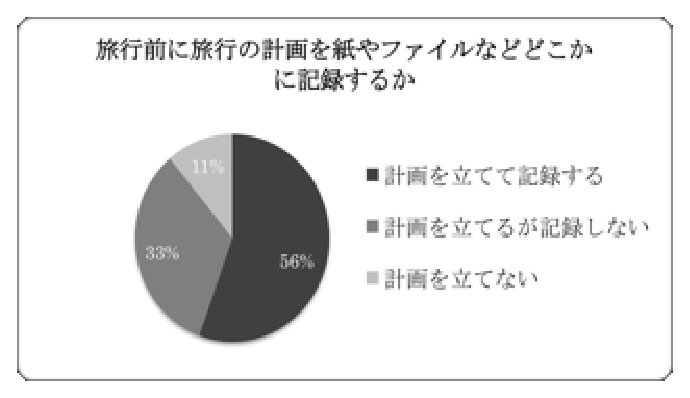
\includegraphics[width=4cm, height=2cm]{filerecord.eps}
\includegraphics[scale=0.7]{ank3.eps}
\caption{旅行計画に関するアンケート(3/6)}
\end{center}
\end{figure}

\begin{figure}[htpb]
\begin{center}
%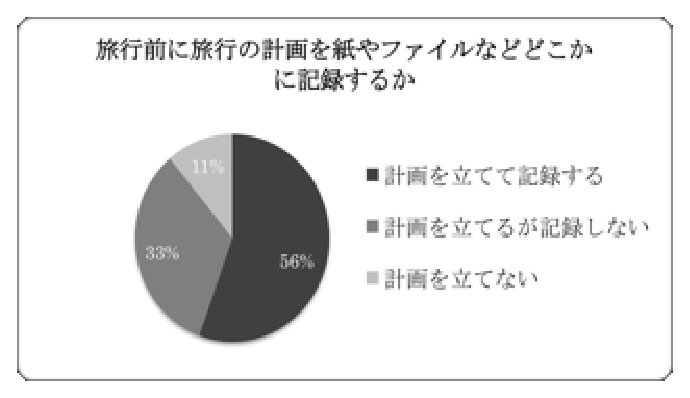
\includegraphics[width=4cm, height=2cm]{filerecord.eps}
\includegraphics[scale=0.7]{ank4.eps}
\caption{旅行計画に関するアンケート(4/6)}
\end{center}
\end{figure}

\begin{figure}[htpb]
\begin{center}
%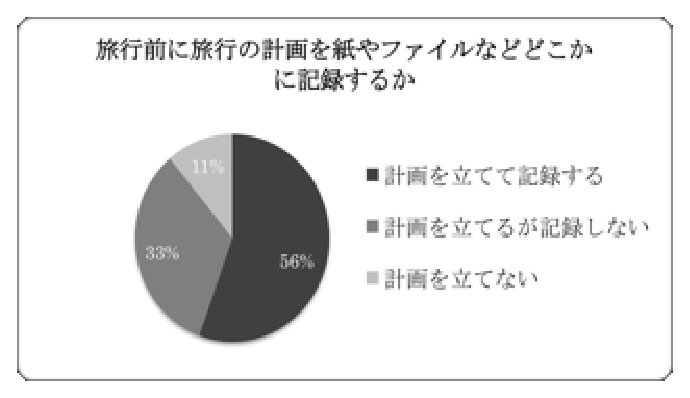
\includegraphics[width=4cm, height=2cm]{filerecord.eps}
\includegraphics[scale=0.7]{ank5.eps}
\caption{旅行計画に関するアンケート(5/6)}
\end{center}
\end{figure}

\begin{figure}[htpb]
\begin{center}
%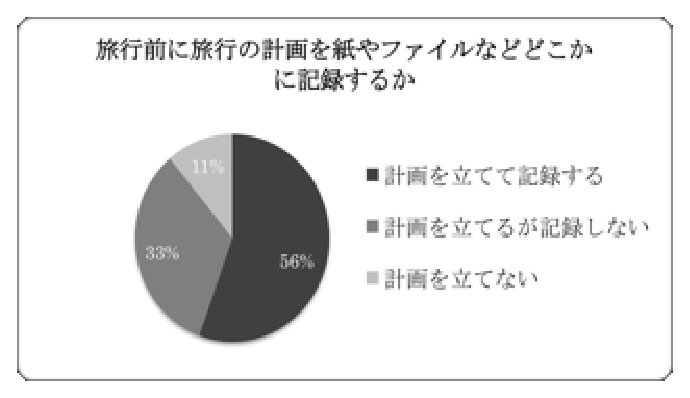
\includegraphics[width=4cm, height=2cm]{filerecord.eps}
\includegraphics[scale=0.7]{ank6.eps}
\caption{旅行計画に関するアンケート(6/6)}
\end{center}
\end{figure}



%--------------------------------------------------------------------
% 図一覧
\listoffigures

%--------------------------------------------------------------------
% 表一覧
\listoftables

\end{document}
